\documentclass[main.tex]{subfiles}

\begin{document}

\chapter{Other contribution} \label{chapter:other_contribution}

This chapter have not any link to other ones they presents about my contribution on some projects where I spent some time during my PhD without sufficiently large contribution to have a specific chapter.

\section{labsquare}

Labsquare is a community for genomics software, this community was create by me and a friend  I participate in developpement of two tools.

\newcommand{\fastqt}{\toolsname{FastQt}}
\newcommand{\cutevariant}{\toolsname{CuteVariant}}

\paragraph{\fastqt} is a rewrite of \toolsname{FastQC} in C++ with the framework \toolsname{Qt}. \fastqt is a tool to check the quality of sequencing data by providing some statistics, GC\% distribution, read length distribution, error rate repartition along the length of reads. At the moment \fastqt development was stopped.

\paragraph{CuteVariant} is a tool to visualize and analyze \toolsname{VCF} (for Variant Call Format) files, these file store variants found between an individual or a dataset of reads against a reference genome. \cutevariant allows selecting annotation, genotype, filter variant, sort and group variants, query variant with \abreviation{VQL} (for Variant Query Language), set operation between VCF file.
\cutevariant is still in development and it was the subject of a poster during the conference Jobim 2019.

\section{CAMI challenge 2}

\abreviation{CAMI} challenge is a metagenomics assembly challenge, I participate in the second edition of CAMI challenge with Camille Marchet, Antoine Limaset, Pierre Peterlongo, Claire Lemaitre and Rayan Chikhi. We tried different strategies to perform an assembly of metagenomics datasets.

\subsection{Dataset description}

In this challenge, we have two datasets with similar reads composition. A set of Illumina Hiseq like reads and a set of Pacbio like reads, simulated by \toolsname{CAMISIM}\cite{camisim}.

We have two dataset, Marine Dataset built to correspond to the composition of a metagenomics sequencing of seawater, and Strain Madness Dataset with very important strain-level variation.

\subsection{Assembly strategy}

On the first hand we perform a short reads assembly with \toolsname{gatb-pipeline} \footnote{https://github.com/GATB/gatb-minia-pipeline}, that is a multi-kmer size short read assembly based on \toolsname{Bloocoo} \cite{bloocoo} for read correction, \toolsname{Minia 3} \cite{minia, bcalm} for contig assembly and \toolsname{BESST} for scaffolding \cite{besst1, besst2, besst3}.

On the second hand, my main contribution in this challenge, we build a long-read assembly pipeline with \toolsname{fmlrc} \cite{fmlrc} a hybrid long-read corrector, and assembly of corrected long read with a pipeline \minimap, \fpa (no internal match and overlap lower than 2000 bases), \miniasm or a \wtdbg assembly. We try to perform read classification before correction and assembly with \toolsname{centrifuge}\cite{centrifuge} to avoid the complexity of metagenomics dataset because our correction assembly tools are not built to use this type of data, but we did not use this strategy due to lack of time.

Finally, we submit a reconciliation of short reads assembly made by \toolsname{gatb-pipeline} and \wtdbg assembly of corrected long-read, if a short reads contig maps in a long reads contig the short reads contigs is discarded. This strategy should have allowed us to have good quality contigs (from long reads assemblies) on the most present strains without losing the information of the least present strains (contained in the short reads contigs). Indeed, long reads sequencing technologies have lower sequencing depths which cannot allow the detection and assembly of the least present strains.

When writing this document, we do not have yet the result  of other team or an idea of quality of our assembly.

\section{10X linked-read deconvolution} \label{section:other_contribution:10x}

10X linked-read was a sequencing technique developed by 10X genomics. Figure \label{fig:other_contribution:10x} present the main idea of 10X linked-read sequencing. After purification DNA was fragmented in large molecule ($\approx$100 kb length), by microfluidic method each large molecule was separate in individuals bubble each bubble was associated with a barcode in this bubble DNA was fragmented in shorter fragment (compatible with Illumina sequencing method) and barcode was add to extremity. After a classic short-read sequencing, we can use barcode information to determinate if read comes from the same large fragment or not.

\begin{figure}
    \centering
    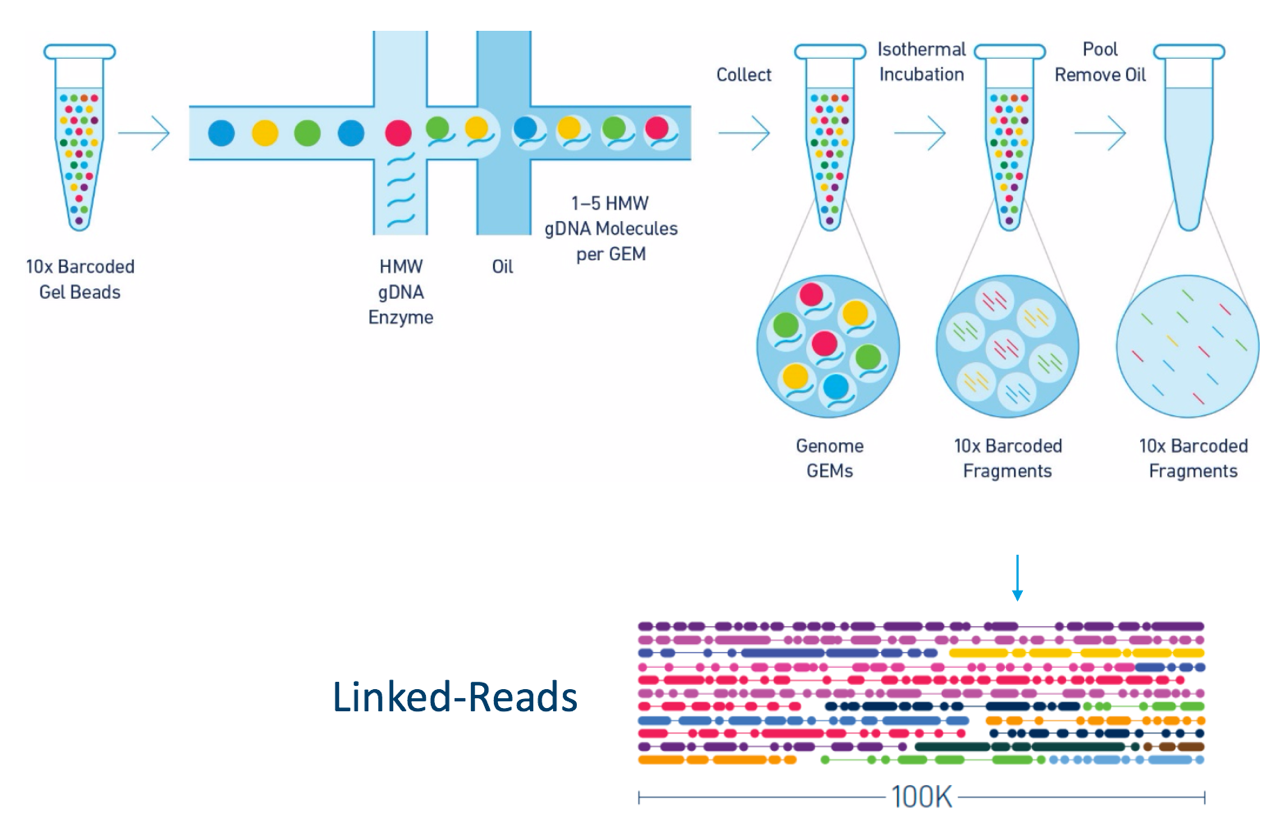
\includegraphics[width=\textwidth]{other_contribution/images/Linked_reads.png}
    \caption{10X linked-read sequencing idea. Source: \url{https://ucdavis-bioinformatics-training.github.io/2018-Dec-Genome-Assembly/10x-supernova/10x-supernova.html}}
    \label{fig:other_contribution:10x}
\end{figure}

Unfortunately, there is not a barcode for each large DNA molecule and therefore several fragments will share the barcode. The task of assigning each reads its original molecule is called deconvolution. Knowing exactly the original molecule of each reads is useful to: 
\begin{itemize}
    \item assembly and scaffollding by allowing to solve repetitions that are span by large molecule
    \item variant phasing all reads come from same molecule, come for same individuals/cells
\end{itemize}
 
If we have access to a good genome reference deconvolution was easy by mapping reads against reference each read with same barcode mapped in approximately 100 kb range on the reference genome come from same molecule, it's general idea used by \toolsname{ema}\cite{ema} and \toolsname{Lariat}\cite{lariat} to assign a read to a molecule.

But when haven't good reference genome we can't use this method. To solve this problem, in colaboration with Chen Sun, Rayan Chikhi , Paul Medvedev and Yoann Dufresne, we try to propose some different techniques to perform a 10x linked-reads deconvolution. I propose a method based on graph assembly analysis.

After a classic \DBG assembly (we use \toolsname{bcalm}), we remap reads against contigs with \toolsname{ema}, to reads with same barcode and map on same contig \toolsname{ema} assign same premolecule identifier. We try to glue premolecule cluster of reads by analyze contigs graph. For all premolecule cluster with same barcode we search shortest path in contigs graph between cluster, if the length (in number of bases) of this path is shortest than a threshold we merge this cluster. 

This method perform some result, but we didn't have time to finish and evaluate methods.

\onlyinsubfile{
\bibliographystyle{plainnat}
\bibliography{main}
\addcontentsline{toc}{chapter}{Bibliography}
}

\end{document}